\documentclass[../../compsys.tex]{subfiles}
\begin{document}
\chapter{File System II}
\vfill
\section{Block Allocation Strategies}
\subsection{Limitations of Traditional Block Allocation}

Files in modern operating systems typically occupy multiple blocks scattered across a disk. This creates several challenges for efficient file access and management:

\begin{itemize}
  \item \textbf{Linked List Approach:} When blocks are linked together, accessing a file requires traversing all preceding blocks.
    \begin{itemize}
      \item If each block access takes 100 $\mu s$, reading 5 blocks requires 500 $\mu s$.
    \end{itemize}
  
  \item \textbf{File Allocation Table (FAT):} To improve performance, systems often cache the FAT in memory.
    \begin{itemize}
      \item This approach consumes significant memory resources.
      \item For each data block, metadata must be stored in the FAT.
      \item Let's analyze the memory and performance implications for a large file:
    \end{itemize}
\end{itemize}

\begin{center}
\fbox{\begin{minipage}{0.95\textwidth}
  \textbf{Memory and Performance Analysis for FAT}\\[0.5em]
  \textbf{Given:}
  \begin{itemize}
    \item File size: 1 TB ($2^{40}$ bytes)
    \item Block size: 4 KB ($2^{12}$ bytes)
    \item FAT entry size: 4 bytes per block (typical)
    \item Block access time: 100 $\mu$s
  \end{itemize}
  
  \textbf{Number of blocks needed to store the file:}
  \begin{align}
    \text{Blocks} &= \frac{\text{File size}}{\text{Block size}} = \frac{1 \text{ TB}}{4 \text{ KB}} = \frac{2^{40} \text{ bytes}}{2^{12} \text{ bytes}}\\
    &= 2^{40-12} = 2^{28} \text{ blocks}
  \end{align}
  
  \textbf{Memory required for FAT entries (metadata):}
  \begin{align}
    \text{FAT size} &= \text{Number of blocks} \times \text{Entry size}\\
    &= 2^{28} \text{ blocks} \times 4 \text{ bytes/block}\\
    &= 2^{28+2} \text{ bytes} = 2^{30} \text{ bytes} = 1 \text{ GB}
  \end{align}
  
  \textbf{Time to access all metadata (worst case):}
  \begin{align}
    \text{Access time} &= \text{Number of metadata blocks} \times \text{Block access time}\\
    &= \frac{1 \text{ GB}}{4 \text{ KB}} \times 100 \text{ $\mu$s} = \frac{2^{30}}{2^{12}} \times 100 \text{ $\mu$s}\\
    &= 2^{18} \times 100 \text{ $\mu$s} \approx 26.2 \text{ seconds}
  \end{align}
  
  \textbf{Implications:} For a 1 TB file, the FAT approach requires 1 GB of memory just to store metadata. Reading all this metadata would take approximately 26 seconds, making file operations extremely slow.
\end{minipage}}
\end{center}

\begin{center}
  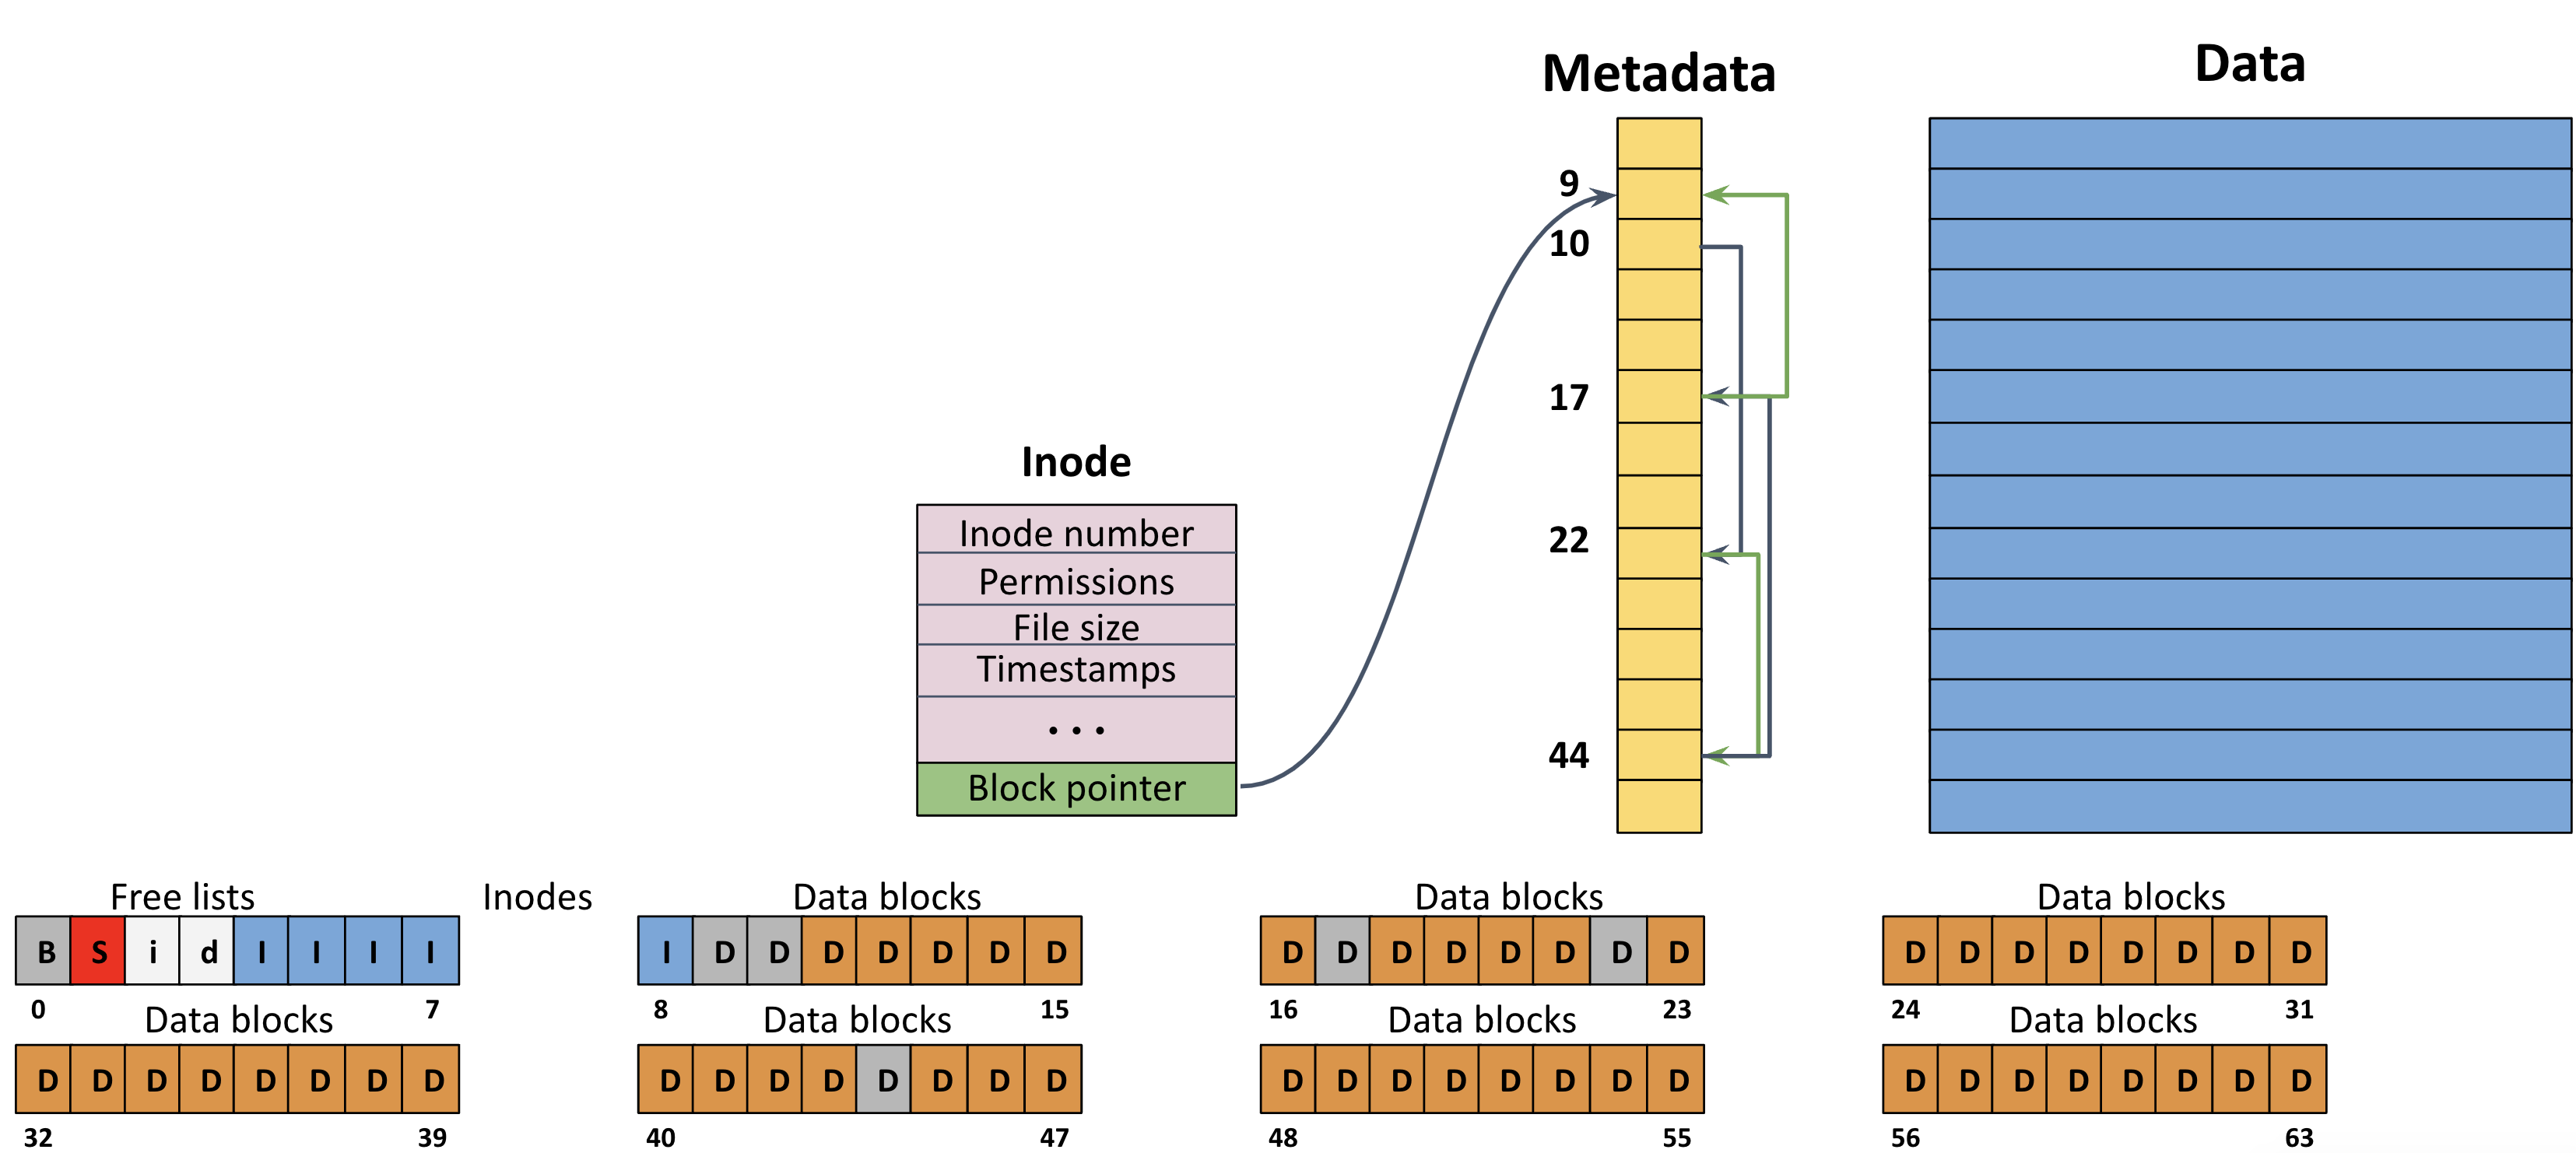
\includegraphics[width=1.05\textwidth]{chapters/L7/images/problem.png}
\end{center}
\newpage
\subsection{Design Goals for Efficient Block Allocation}

A well-designed block allocation strategy should balance several competing requirements:
\begin{itemize}
  \item Minimize memory overhead for metadata
  \item Provide fast access to all parts of a file
  \item Support both small and large files efficiently
  \item Scale gracefully as file size increases
\end{itemize}

\subsection{The Inode Approach}

\noindent
\begin{minipage}{0.55\textwidth}
  \textbf{Key Observation:} File systems must efficiently handle two common types of files:
  
  \begin{enumerate}
    \item \textbf{Small files} ($<$ 50 KB)
      \begin{itemize}
        \item Can be accessed directly with a small set of pointers
        \item Direct inode pointers point to data blocks
      \end{itemize}
    
    \item \textbf{Large files}
      \begin{itemize}
        \item Metadata blocks are allocated as the file grows
        \item Similar to multi-level page tables
        \item Minimizes memory waste through indirection
      \end{itemize}
  \end{enumerate}
\end{minipage}
\hfill
\vline
\hfill
\begin{minipage}{0.35\textwidth}
  \begin{center}
    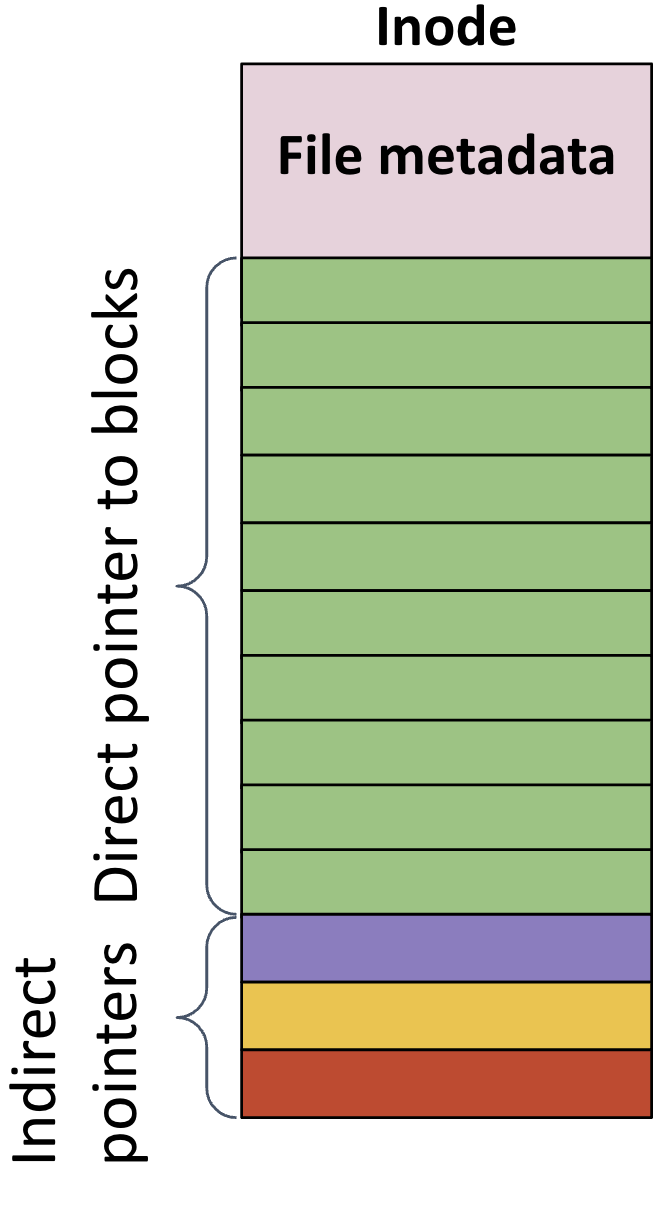
\includegraphics[width=0.85\textwidth]{chapters/L7/images/inode.png}
  \end{center}
\end{minipage}
 
\begin{center}
  \textbf{Inode Pointer Structure}\\[0.5em]
  An inode contains a fixed set of pointers that provide access to data blocks using a hierarchical addressing scheme:
  
  \begin{tabularx}{\textwidth}{|C{0.23\textwidth}|X|C{0.23\textwidth}|}
    \hline
    \textbf{Pointer Type} & \textbf{Description} & \textbf{File Size Range} \\
    \hline
    \textbf{Direct} & 
    First 12 pointers point directly to data blocks, providing immediate, single-step access with no indirection overhead. 
    & Small files ($\leq$ 48 KB) \\
    \hline
    \textbf{Single-Indirect} & 
    Pointer \#13 points to a block of pointers where each entry points to a data block (one level of indirection). 
    & Medium files (up to several MB) \\
    \hline
    \textbf{Double-Indirect} & 
    Pointer \#14 points to a block of pointers; each entry in that block points to another block, which in turn contains pointers to data blocks (two levels of indirection). 
    & Large files (up to several GB) \\
    \hline
    \textbf{Triple-Indirect} & 
    Pointer \#15 points to a block of pointers; each entry points to another block of pointers, then to yet another block before finally reaching data blocks (three levels of indirection). 
    & Very large files (up to TB range) \\
    \hline
    \end{tabularx}
\end{center}

\subsection{Benefits of the Inode Structure}
\begin{itemize}
  \item \textbf{Space Efficiency:} Metadata grows only as needed for larger files
  \item \textbf{Access Speed:} Small files can be accessed with minimal indirection
  \item \textbf{Scalability:} Can address extremely large files with limited overhead
  \item \textbf{Balanced Approach:} Optimizes for both small and large file access patterns
\end{itemize}


\section{File Allocation Approach: Multi-level Indexing}

The multi-level indexing scheme employs a tree-like structure to organize file data blocks, enhancing the efficiency of block retrieval. This approach uses a combination of direct, single indirect, double indirect, and triple indirect pointers to reference data blocks, thereby adapting the indexing depth to the file size.

\subsection*{Key Features and Advantages}

\begin{itemize}
    \item \textbf{Efficient Block Location:} The tree structure allows rapid location of data blocks. Once an indirect block is read, it can reference hundreds of data blocks, making sequential read operations highly efficient.
    
    \item \textbf{Asymmetric Overhead:} The design is asymmetric, meaning that small files benefit from minimal overhead by primarily using direct pointers, while larger files leverage additional levels of indirection without incurring a prohibitive metadata cost.
    
    \item \textbf{Fixed Structure and Simplicity:} The fixed, hierarchical layout simplifies implementation. Metadata is stored separately from data, ensuring there is no conflation between file data and file system metadata.
    
    \item \textbf{No External Fragmentation:} Since data blocks are allocated without external fragmentation, the overall space utilization is improved.
    
    \item \textbf{Performance:} The structure provides reasonable read performance with low seek times, balancing the extra reads required for indirect accesses with the overall efficiency of accessing multiple blocks once an indirect block is in memory.
\end{itemize}

\subsection*{Dynamic Allocation and Practical Considerations}

The allocation dynamics are designed to be adaptive:

\begin{itemize}
    \item \textbf{Small Files:} For a file that contains only a few kilobytes of data, direct pointers are used. For example, reading a 4~KB block from a file accessed via a direct pointer incurs minimal overhead.
    
    \item \textbf{Large Files:} As the file size grows, additional levels of indexing are activated. With a three-level (triple indirect) indexing, even a file requiring 16~KB of data can be managed efficiently. The extra levels allow the file system to scale, enabling support for very large files without a linear increase in metadata.
    
    \item \textbf{Mixed Access Patterns:} The tree-like indexing provides a good balance between random access (via direct pointers) and sequential reads (via high-degree indirect blocks), which is beneficial for different file access patterns.
\end{itemize}

\begin{center}
  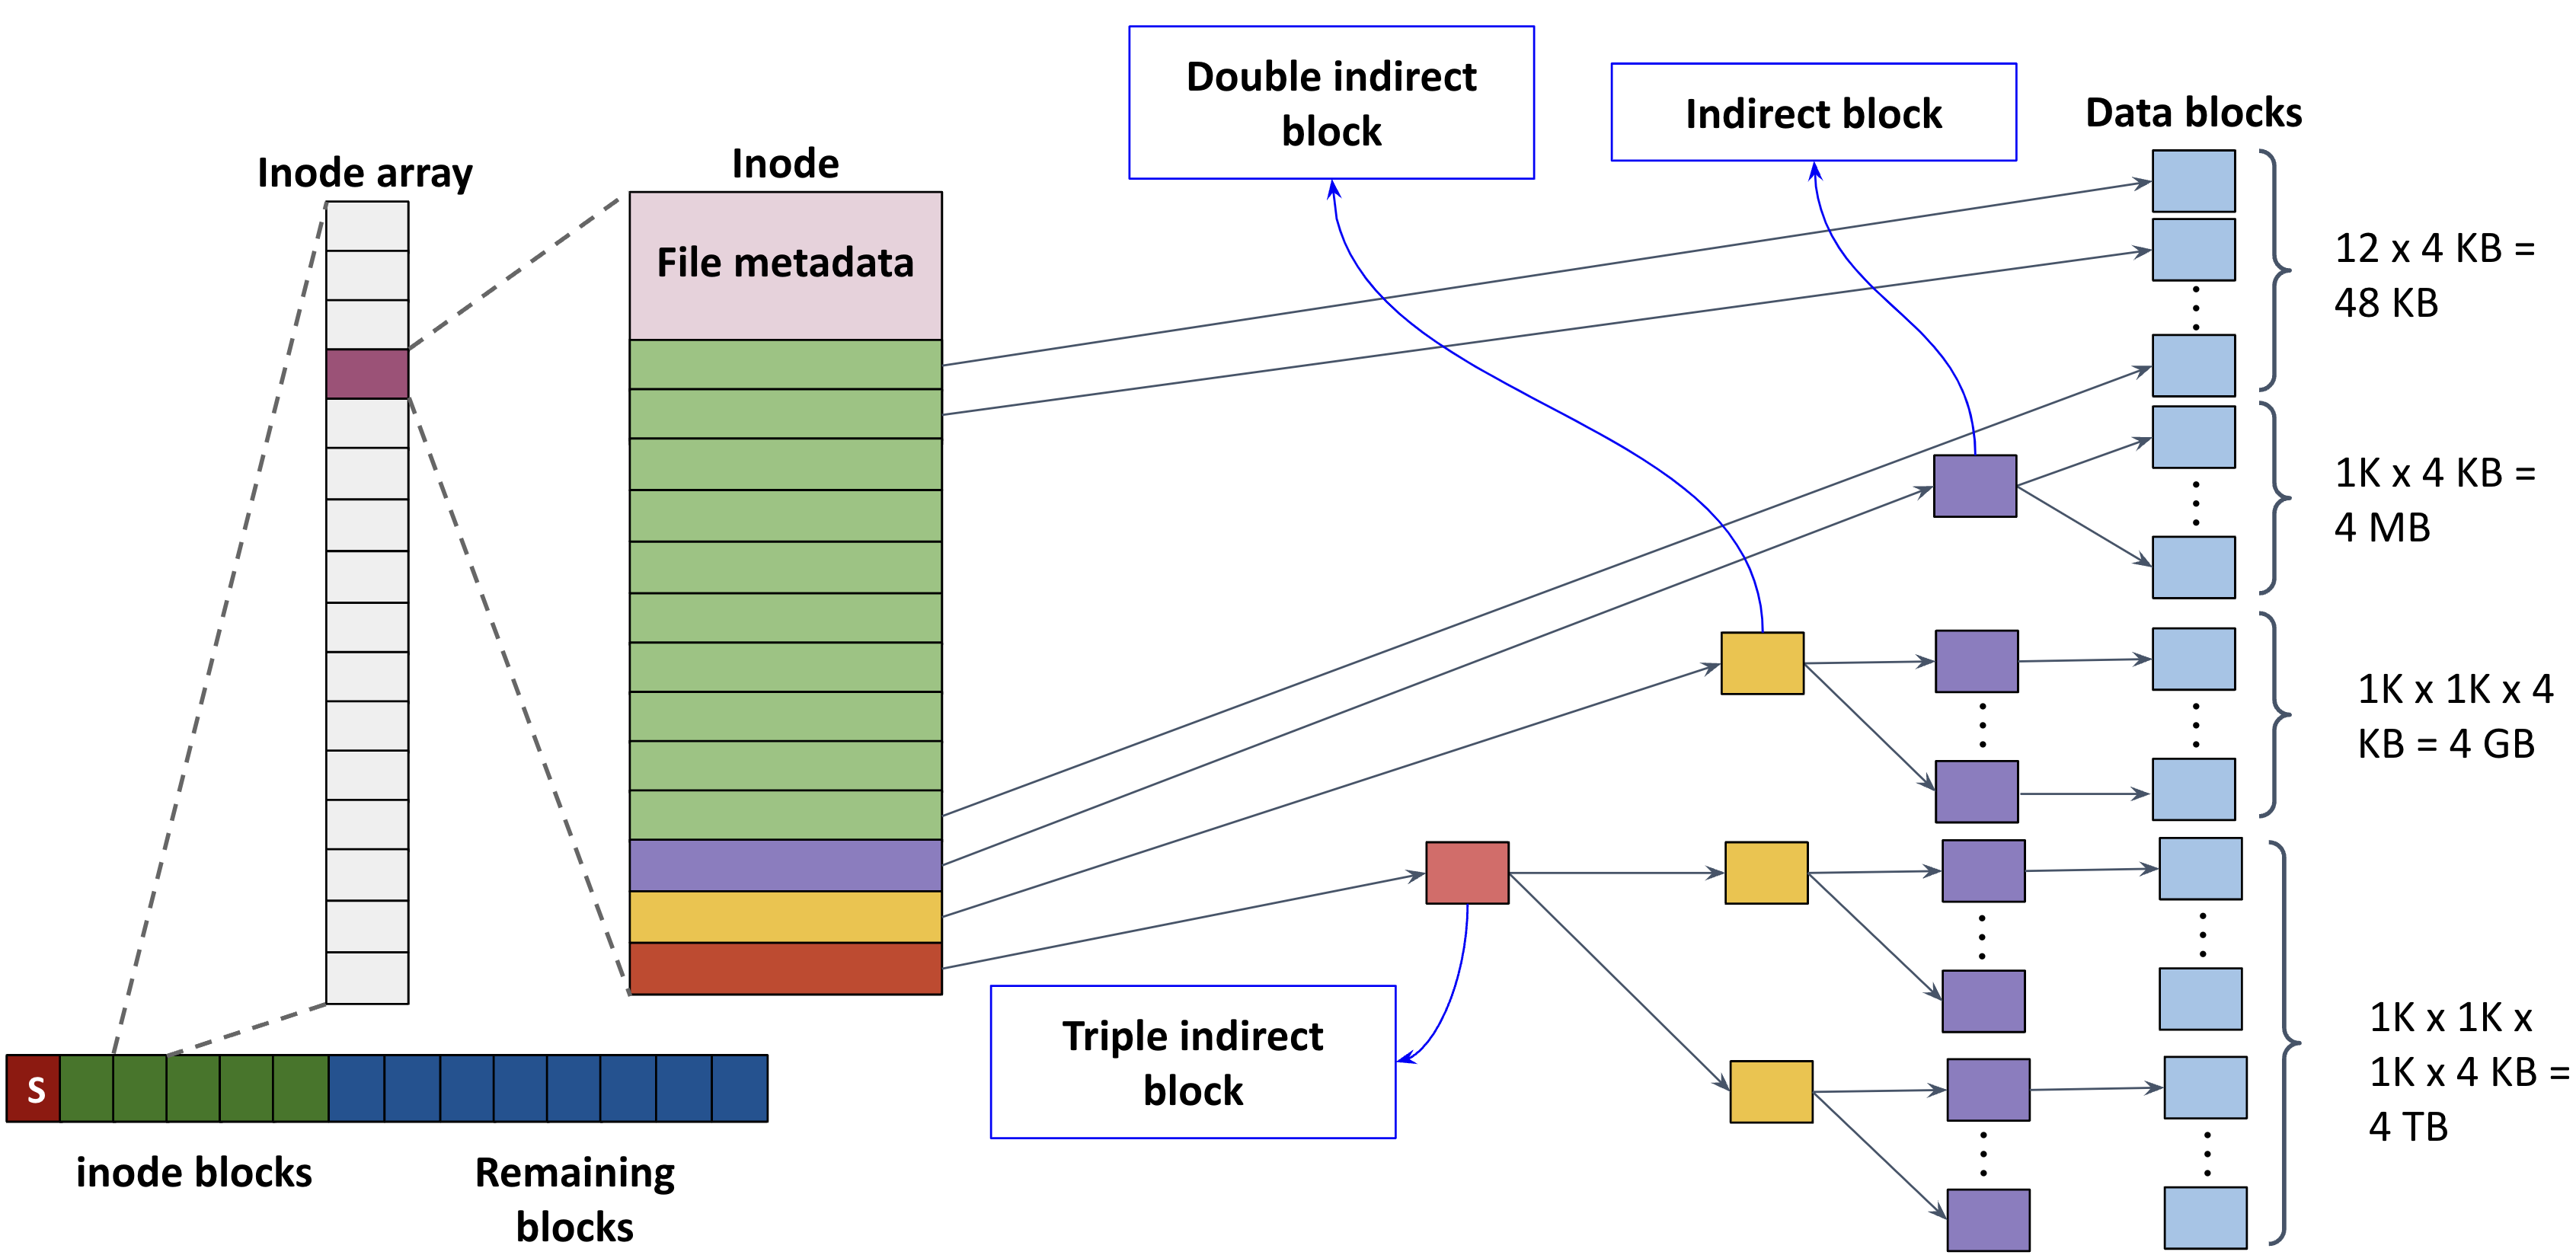
\includegraphics[width=0.8\textwidth]{chapters/L7/images/multi.png}
\end{center}
The multi-level indexing file allocation method enhances both performance and scalability by adapting the index structure to the file size, ensuring low overhead for small files while supporting efficient access for large files.


\newpage
\section{File Operations in a Filesystem}

Reading and writing files in a filesystem involve complex sequences of operations that extend beyond simply accessing data. These operations require traversing directory structures, accessing metadata, and managing disk blocks. This section explores the mechanics of these fundamental operations.

\subsection{Reading from a File}
When an application reads data from a file, the operating system performs multiple disk operations to locate and retrieve the requested data. The process begins with opening the file and continues with reading data blocks as needed.

\subsubsection{Opening a File for Reading}
Before data can be read, the file must be opened:

\begin{example}[Opening a file]
\texttt{open("/cs202/w07", O\_RDONLY)}
\end{example}

This system call initiates a sequence of operations:
\begin{itemize}
    \item The filesystem traverses the directory tree to locate the inode for "w07"
    \item It reads the inode to verify access permissions
    \item Upon successful verification, it returns a file descriptor that serves as a reference for subsequent operations
\end{itemize}

\subsubsection{Reading Data}
Each \texttt{read()} operation requires multiple steps:
\begin{itemize}
    \item The filesystem reads the file's inode to locate the appropriate data blocks
    \item It reads the data block(s) corresponding to the current file offset
    \item It updates the last access time in the inode
    \item It updates the file offset in the in-memory open file table for the file descriptor
\end{itemize}
\newpage
\begin{example}[Reading the First Two Data Blocks from "/cs202/w07"]
\leavevmode
\upshape
Let's look at the complete sequence of operations required to open a file and read its first two data blocks.

\textbf{Step 1: Opening the File}
\begin{enumerate}
    \item \textbf{Root inode access:} The system reads the inode of the root directory (/) to locate its data blocks.
    
    \item \textbf{Root directory data:} The filesystem reads the root directory's data blocks to find the entry for "cs202".
    
    \item \textbf{cs202 inode access:} Using information from the root directory, it reads the inode for the "cs202" subdirectory.
    
    \item \textbf{cs202 directory data:} It reads the data blocks of the "cs202" directory to locate the entry for "w07".
    
    \item \textbf{w07 inode access:} Finally, it reads the inode associated with "w07", which contains the metadata and pointers to the file's data blocks.
\end{enumerate}

At this point, the file is open and the system has established the necessary references to access its data.

\textbf{Step 2: First read() Call}
\begin{enumerate}
    \item \textbf{w07 inode read:} The system reads the inode again to retrieve the pointer to the first data block and verify metadata.
    
    \item \textbf{Data block access:} It reads the actual first data block of file "w07".
    
    \item \textbf{Inode update:} It writes to the inode to update the last access timestamp.
\end{enumerate}

\textbf{Step 3: Second read() Call}
\begin{enumerate}
    \item \textbf{w07 inode read:} The system reads the inode again to retrieve the pointer to the second data block.
    
    \item \textbf{Data block access:} It reads the second data block of file "w07".
    
    \item \textbf{Inode update:} It writes to the inode to update the last access timestamp again.
\end{enumerate}
\end{example}

The sequence of operations for file reads can be visualized as follows:

\begin{center}
  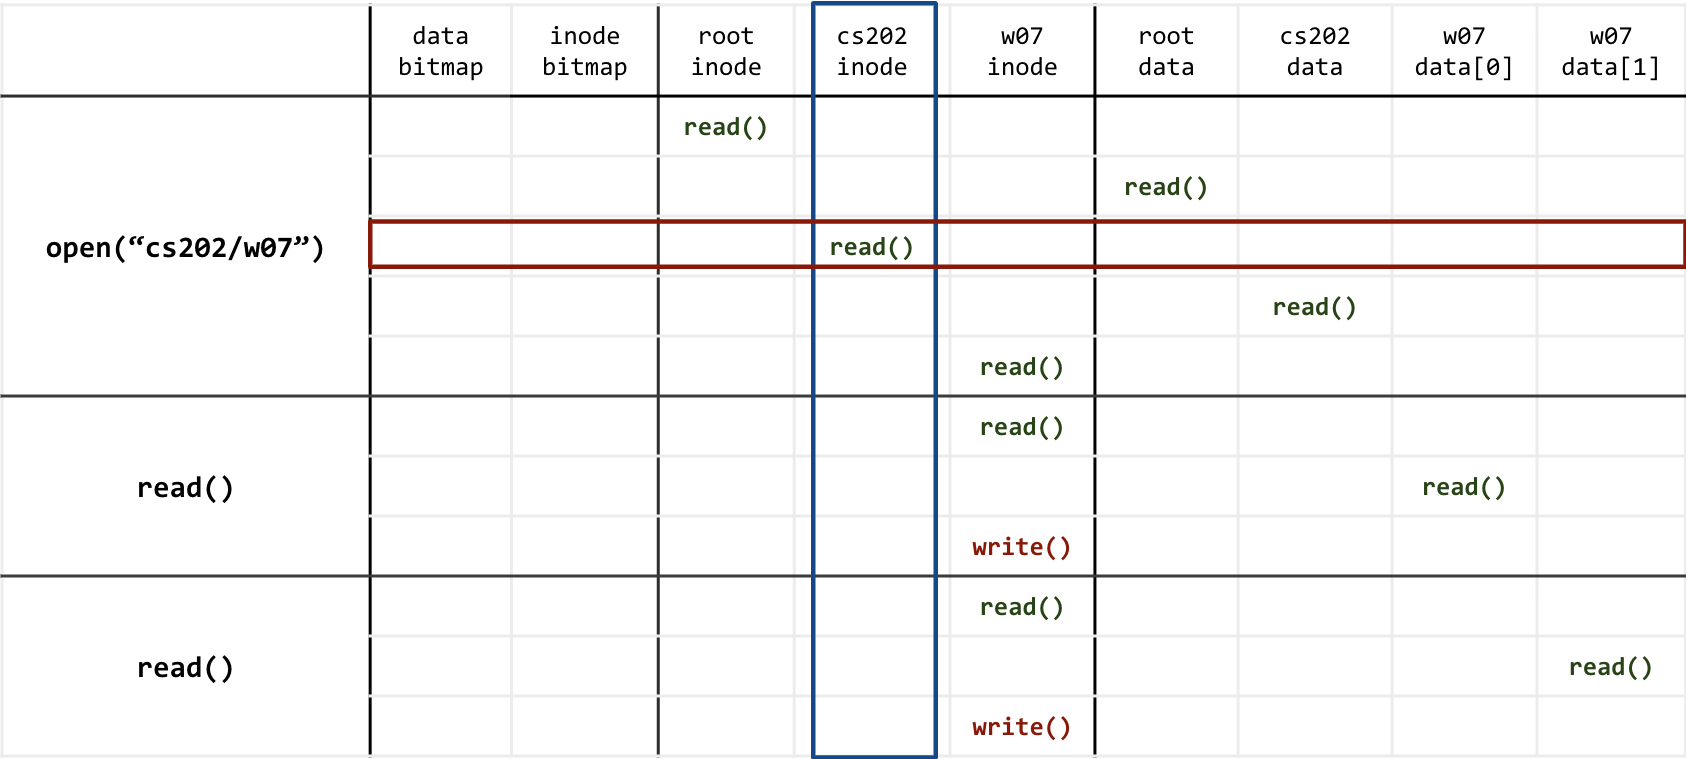
\includegraphics[width=0.8\textwidth]{chapters/L7/images/read.png}
\end{center}

\subsection{Writing to a File}
Writing to a file involves more complex operations than reading, particularly when new data blocks need to be allocated.

\subsubsection{Opening a File for Writing}
Similar to reading, writing begins with opening the file:

\begin{example}[Opening a file for writing]
\texttt{open("/cs202/w07", O\_WRONLY)}
\end{example}

This assumes the file already exists. If it doesn't, additional operations would be required to create it.

\subsubsection{Writing Data}
Each logical write operation can generate multiple physical I/O operations:

\begin{enumerate}
    \item Read the free data block bitmap to locate available space
    \item Write to the data block bitmap to mark the block as allocated
    \item Read the file's inode to access its metadata
    \item Write to the file's inode to update its block pointers
    \item Write the actual data to the newly allocated block
\end{enumerate}

\subsubsection{File Creation and Additional Complexity}
Creating a new file involves even more operations:
\begin{itemize}
    \item Reading and writing the free inode bitmap to allocate an inode
    \item Writing the new inode with initial metadata
    \item Reading and updating the parent directory's data blocks
    \item If the parent directory is full, allocating new blocks for it
\end{itemize}
\newpage
\begin{example}[Creating and Writing to a New File "/cs202/w07"]
\leavevmode
\upshape
Now, let's look at the complete sequence of operations required to create a new file and write its first data block.

\begin{center}
  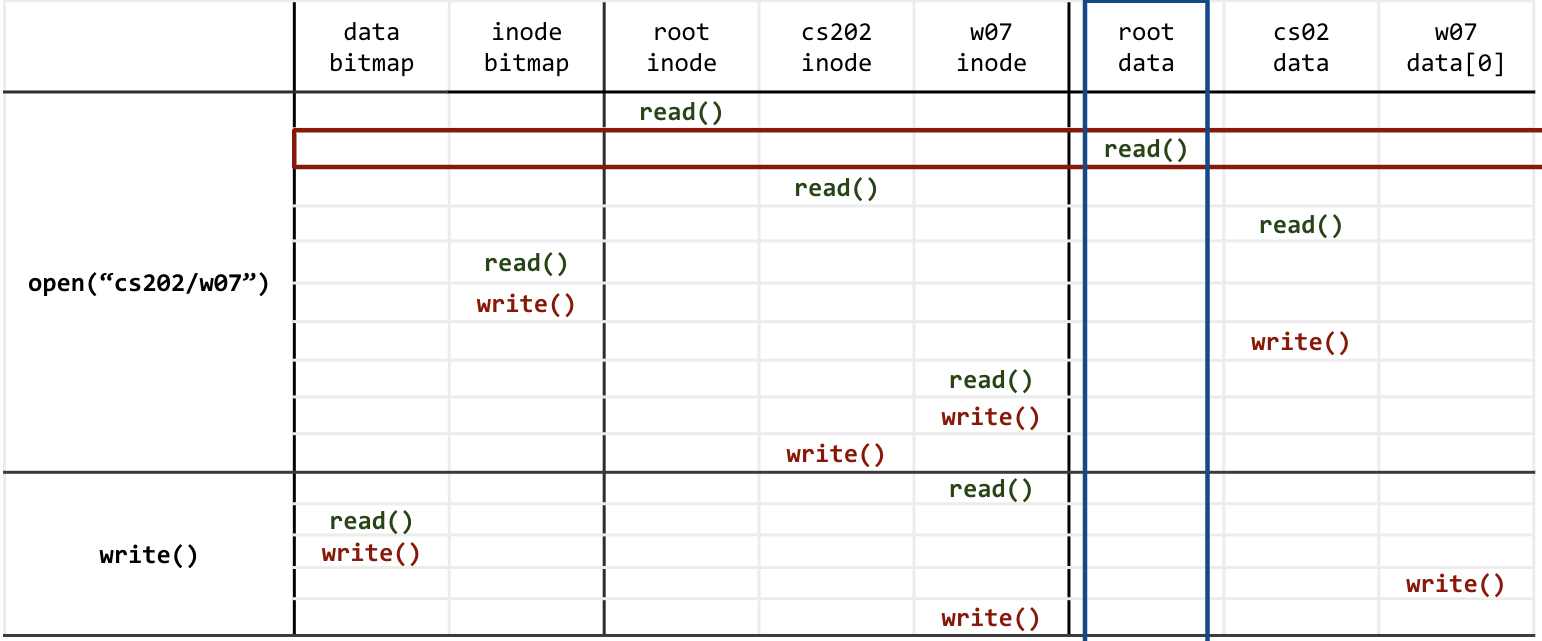
\includegraphics[width=0.8\textwidth]{chapters/L7/images/write.png}
\end{center}
\textbf{Step 1: Creating the File}
\begin{enumerate}
    \item \textbf{Root inode access:} Reads the root directory's inode to locate its data blocks.
    
    \item \textbf{Root directory data:} Reads the root directory's data to find the entry for "cs202".
    
    \item \textbf{cs202 inode access:} Reads the inode for the "cs202" directory.
    
    \item \textbf{cs202 directory data:} Reads "cs202" directory data to verify "w07" doesn't already exist.
    
    \item \textbf{Inode bitmap operations:} Reads the inode bitmap to find a free inode, then writes to mark it as allocated.
    
    \item \textbf{Directory update:} Updates the "cs202" directory data to include an entry for "w07" linked to the new inode.
    
    \item \textbf{New inode initialization:} Writes initial metadata to the new inode (permissions, owner, timestamps).
    
    \item \textbf{Parent directory update:} Updates the metadata for "cs202" (modification time, entry count).
\end{enumerate}

\textbf{Step 2: Writing Data to the New File}
\begin{enumerate}
    \item \textbf{w07 inode access:} Reads the new file's inode to access its metadata.
    
    \item \textbf{Data bitmap operations:} Reads the data bitmap to find a free data block, then writes to mark it as allocated.
    
    \item \textbf{Data write:} Writes the actual file content to the newly allocated data block.
    
    \item \textbf{Inode update:} Updates the "w07" inode with the new file size, data block pointers, and timestamps.
\end{enumerate}
\end{example}
\newpage
\section{File System Performance}

File system performance is a critical aspect of operating system design that directly impacts user experience and application efficiency. This section explores how performance is defined, measured, and optimized in file systems.

\subsection{Performance Metrics and Evaluation}

Performance in file systems can be evaluated from multiple perspectives, each focusing on different aspects of system behavior:

\begin{definition}[File System Performance]
The measure of how efficiently a file system can execute operations such as reading, writing, and metadata manipulation, typically expressed in terms of latency, throughput, and resource utilization.
\end{definition}

When evaluating file system performance, several factors must be considered:

\begin{itemize}
  \item \textbf{Operation count:} The number of I/O operations required to complete a task
  \item \textbf{Operation speed:} The time required to complete individual I/O operations
  \item \textbf{Program-level impact:} Effect on the performance of a single program
  \item \textbf{System-level impact:} Effect on overall system performance across all programs
\end{itemize}

These factors can be quantified using the following key metrics:

\begin{itemize}
  \item \textbf{Latency:} The time delay between initiating and completing an operation
  \item \textbf{Throughput:} The amount of data processed per unit time (e.g., MB/s)
  \item \textbf{IOPS (I/O Operations Per Second):} The number of read/write operations a storage system can perform in one second
\end{itemize}
\newpage
\subsection{Performance Optimization Strategies}

File systems employ various strategies to optimize performance, each addressing different performance bottlenecks \\[5px]

\begin{definition}[Block Cache]
A memory area that temporarily stores recently accessed disk blocks to reduce the need for physical disk operations when the same data is requested again.
\end{definition}

Caching significantly improves performance by reducing the need for slow disk operations:
\begin{itemize}
  \item[-] Frequently accessed blocks remain in memory, allowing \texttt{read()} operations to complete without disk I/O
  \item[-] Modern systems often dedicate all unused memory to the file system buffer cache
  \item[-] The cache maps file identifiers (inode, block offset) to physical memory locations (page frame numbers)
\end{itemize}

\subsubsection{Operation Batching}
Grouping multiple operations together can significantly improve overall system throughput:

\begin{example}[Write Batching]
Instead of writing data to disk immediately after each user interaction, an application can queue multiple write operations for 5 seconds and then perform them as a batch. This reduces the total number of disk accesses, improving throughput at the cost of slightly increased latency for individual operations.
\end{example}

The benefits of operation batching include:
\begin{itemize}
  \item[-] Reduced disk seek time by grouping operations on physically proximate disk sectors
  \item[-] Amortized per-operation overhead across multiple operations
  \item[-] Opportunity for operation optimization and reordering
\end{itemize}

\subsubsection{Delayed Idempotent Operations}

\begin{definition}[Idempotent Operation]
An operation that can be performed multiple times without changing the final outcome beyond the initial application.
\end{definition}

Delaying or batching idempotent operations provides performance benefits without compromising correctness:

\begin{example}[Timestamp Updates]
Updating a file's "last accessed" timestamp can be delayed or batched because only the most recent timestamp is relevant. Multiple updates within a short time window can be coalesced into a single disk write.
\end{example}

\subsubsection{Strategic Indirection}

Adding levels of indirection enables optimization opportunities:
\begin{itemize}
  \item Maintaining abstractions that decouple logical operations from physical ones
  \item Allowing the system to reorder or coalesce operations
  \item Providing flexibility in how and when operations are physically executed
\end{itemize}
\newpage
\subsection{The Block Cache Architecture}
The block cache serves as a critical performance optimization layer in file systems\\[5px]

\begin{example}[Block Cache Operation]
\leavevmode
\upshape
\noindent When an application repeatedly reads the same inode block\\[9px]
\begin{minipage}{0.45\textwidth}
\begin{enumerate}
  \item \textbf{First read:} The block is loaded from disk into the block cache
  \item \textbf{Subsequent reads:} The system checks if the block is in the cache using the mapping:
  $\{inode, block\_offset\} \rightarrow page\_frame\_number$
  \item If found, the data is returned directly from memory without disk I/O
  \item The block remains in cache until memory pressure forces eviction
\end{enumerate}
\end{minipage}
\hfill
\vline
\hfill
\begin{minipage}{0.45\textwidth}
  \begin{center}
    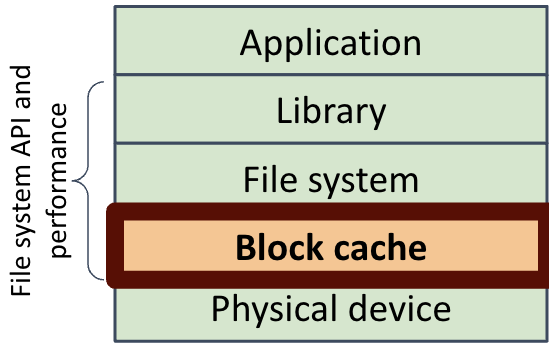
\includegraphics[width=0.75\textwidth]{chapters/L7/images/layers.png}
  \end{center}
\end{minipage}
\end{example}
\vspace{10px}
\subsubsection{Key Block Cache Characteristics}
\begin{itemize}
  \item[-] Dynamically adjusts size based on system memory availability
  \item[-] Implements replacement policies to maximize cache hit rates
  \item[-] Manages consistency between cached blocks and their disk versions
  \item[-] May implement read-ahead or prefetching to anticipate future access patterns
\end{itemize}

These performance optimization strategies collectively ensure that file systems can deliver high throughput and low latency despite the inherent performance limitations of physical storage devices.
\newpage
\subsection{Optimizing I/O Operations Through Batching}

\begin{definition}[I/O Batching]
The process of combining multiple I/O operations into larger, more efficient transfers to minimize overall system overhead and maximize throughput.
\end{definition}

Modern file systems employ batching strategies to address two key performance limitations:
\begin{itemize}
    \item High latency cost per individual I/O operation
    \item Limited I/O operations per second (IOPS) capacity
\end{itemize}

\subsubsection{Storage-Specific Optimizations}

Different storage technologies benefit from distinct batching strategies:

\begin{itemize}
    \item \textbf{Hard Disk Drives (HDD):}
    \begin{itemize}
        \item Optimizes for sequential access by grouping operations on consecutive disk blocks
        \item Minimizes seek time by processing physically proximate blocks together
        \item Performance heavily influenced by disk fragmentation - the degree to which an inode's blocks are non-contiguous
    \end{itemize}
    
    \item \textbf{Solid State Drives (SSD):}
    \begin{itemize}
        \item Leverages internal parallelism for concurrent operations
        \item Benefits from larger transfer sizes due to internal architecture
        \item Less sensitive to physical block placement
    \end{itemize}
\end{itemize}

\subsection{Asynchronous Operations and Write Delays}

While read operations typically require immediate process blocking, write operations present opportunities for optimization through delayed execution:

\begin{example}[Asynchronous Write Operations]
When an application writes data:
\begin{enumerate}
    \item Data is initially stored in memory buffers
    \item Write operations are queued for asynchronous processing
    \item System performs actual disk writes within a defined interval (typically 30 seconds)
    \item Operations may be reordered to optimize throughput
\end{enumerate}
\end{example}
\vspace{10px}
\begin{definition}[Write Delay]
A performance optimization technique where write operations are temporarily held in memory and executed asynchronously to improve system throughput.
\end{definition}
\vspace{5px}

\textbf{Important Note:} While write delays improve performance, they introduce a risk of data loss in case of system crashes before cached data is written to disk.

\subsection{Cache Impact on Data Persistence}
File systems cache multiple critical data structures to enhance performance:
\begin{itemize}
    \item[-] Free block and inode bitmaps
    \item[-] Directory entries
    \item[-] Inode metadata
    \item[-] Data blocks
\end{itemize}

While caching significantly improves read performance, it introduces complexity for write operations due to the need to maintain data consistency between memory and disk.

\subsection{Write Caching Policies}
File systems implement different caching strategies to balance performance and data consistency:
\vspace{5px}
\begin{definition}[Write-Back Cache]
A caching policy where modifications are initially made to the cache and later written to disk, prioritizing performance over immediate consistency.
\end{definition}
\vspace{5px}
\begin{definition}[Write-Through Cache]
A caching policy where modifications are immediately written to both cache and disk, ensuring consistency at the cost of performance.
\end{definition}

\begin{center}
\begin{tabular}{|l|l|l|}
\hline
\textbf{Cache Policy} & \textbf{Advantages} & \textbf{Disadvantages} \\
\hline
Write-Back & Higher performance & Risk of data loss \\
& Better I/O optimization & during system crashes \\
\hline
Write-Through & Guaranteed consistency & Lower performance \\
& Immediate persistence & Higher I/O overhead \\
\hline
\end{tabular}
\end{center}

Applications can force immediate disk writes using the \texttt{fsync} system call when data consistency is critical.

\section{Crash Consistency}

Suppose we are appending a data block to a file. This operation involves several steps: adding a new data block \( D2 \), updating the inode, and updating the data bitmap.

\begin{center}
  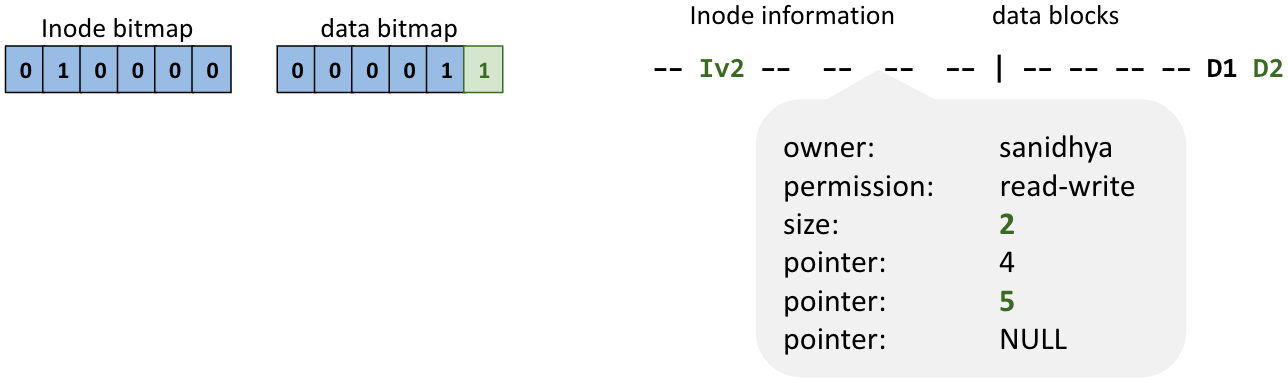
\includegraphics[width=0.8\textwidth]{chapters/L7/images/update.png}
\end{center}

What happens if a crash or power outage occurs during these writes? The key issue is that file system operations often involve multiple write operations, and a failure between these operations can lead to an inconsistent state.

\subsection{Single Write Scenario}

Consider the case where only one write operation is successfully written to disk before a crash. Let's examine a few possibilities:

\begin{itemize}
    \item \textbf{Data Block \( D2 \) is written}: The data is written, but there is no valid inode pointing to it. \( D2 \) appears as a free block in the metadata. The write is essentially lost, but the file system metadata structures remain consistent.
    \item \textbf{Inode ( \( Iv2 \) ) is written}: If only the updated inode \( Iv2 \) is written, following the block pointer will lead to reading garbage data. This results in an inconsistent file system because the data bitmap indicates that the block is free, while the inode claims it is in use.
    \item \textbf{Updated Data Bitmap is written}: If only the updated data bitmap is written, the file system becomes inconsistent because the data bitmap indicates that a data block is in use, but no inode points to it.
\end{itemize}

\begin{center}
  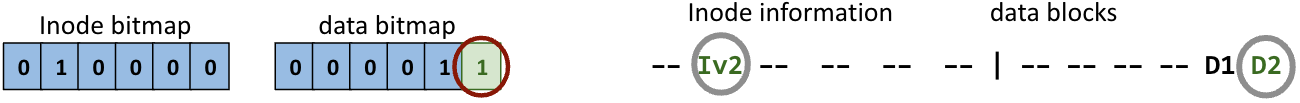
\includegraphics[width=0.8\textwidth]{chapters/L7/images/single-write.png}
\end{center}

\subsection{Multiple Writes Scenario}

Now, let's consider scenarios where two write operations succeed before a crash:

\begin{itemize}
    \item \textbf{Inode and Data Bitmap updates succeed}: The file system remains consistent from a metadata perspective. However, reading the new block will return garbage data because the actual data block \( D2 \) was not successfully written.
    \item \textbf{Inode and Data Block updates succeed}: This leads to an inconsistent file system because the inode points to the new data block, but the data bitmap might not reflect that the block is in use.
    \item \textbf{Data Bitmap and Data Block updates succeed}: This also results in an inconsistent file system because the data bitmap marks the data block as used, but no inode points to it.
\end{itemize}

Caching exacerbates these issues because data can be written asynchronously, making it harder to predict the order of writes.

If the file system is interrupted between these writes, it can lead to an inconsistent state due to:

\begin{itemize}
    \item Power loss and hard reboot
    \item Kernel panic
    \item File system bugs
\end{itemize}

Therefore, a mechanism is needed to recover from or fix these inconsistent states.
\newpage
\subsection{The Consistent Update Problem}

The fundamental problem is that several file system operations update multiple data structures. Caching can worsen the issue because data can be written asynchronously. If a file system operation is interrupted between writes, it may leave the data in an inconsistent state. This can occur due to power loss, hard reboots, kernel panics, or file system bugs.

Therefore, the goal is to have a mechanism to recover from (or fix) an inconsistent state.

\subsection{Consistency Solution \#1: File System Checker (FSCK)}

One approach to address file system inconsistencies is using a file system checker (FSCK). FSCK is a utility that checks the consistency of the file system after a certain number of mount operations or after a crash. It performs hundreds of consistency checks across different fields, such as:

\begin{itemize}
    \item Do superblocks match?
    \item Is the file system size reasonable?
    \item Are link counts equal to the number of directory entries?
\end{itemize}
\subsection{The File System Checker}

The file system checker (\texttt{fsck}) is a crucial utility for maintaining file system integrity. It is automatically invoked after a specific number of mount operations or following a system crash to ensure the file system's consistency. The \texttt{fsck} performs numerous checks across various file system components, addressing potential issues like incorrect link counts, data bitmap errors, duplicate pointers, and invalid pointers.

The following are examples of the consistency checks \texttt{fsck} performs:

\begin{itemize}
    \item [-] \textbf{Link Count Inconsistencies:}
    The \texttt{fsck} verifies that the number of directory entries pointing to an inode matches the inode's link count. For instance, if two directory entries point to the same inode but the inode's link count is set to 1, \texttt{fsck} detects this inconsistency.
    \begin{center}
        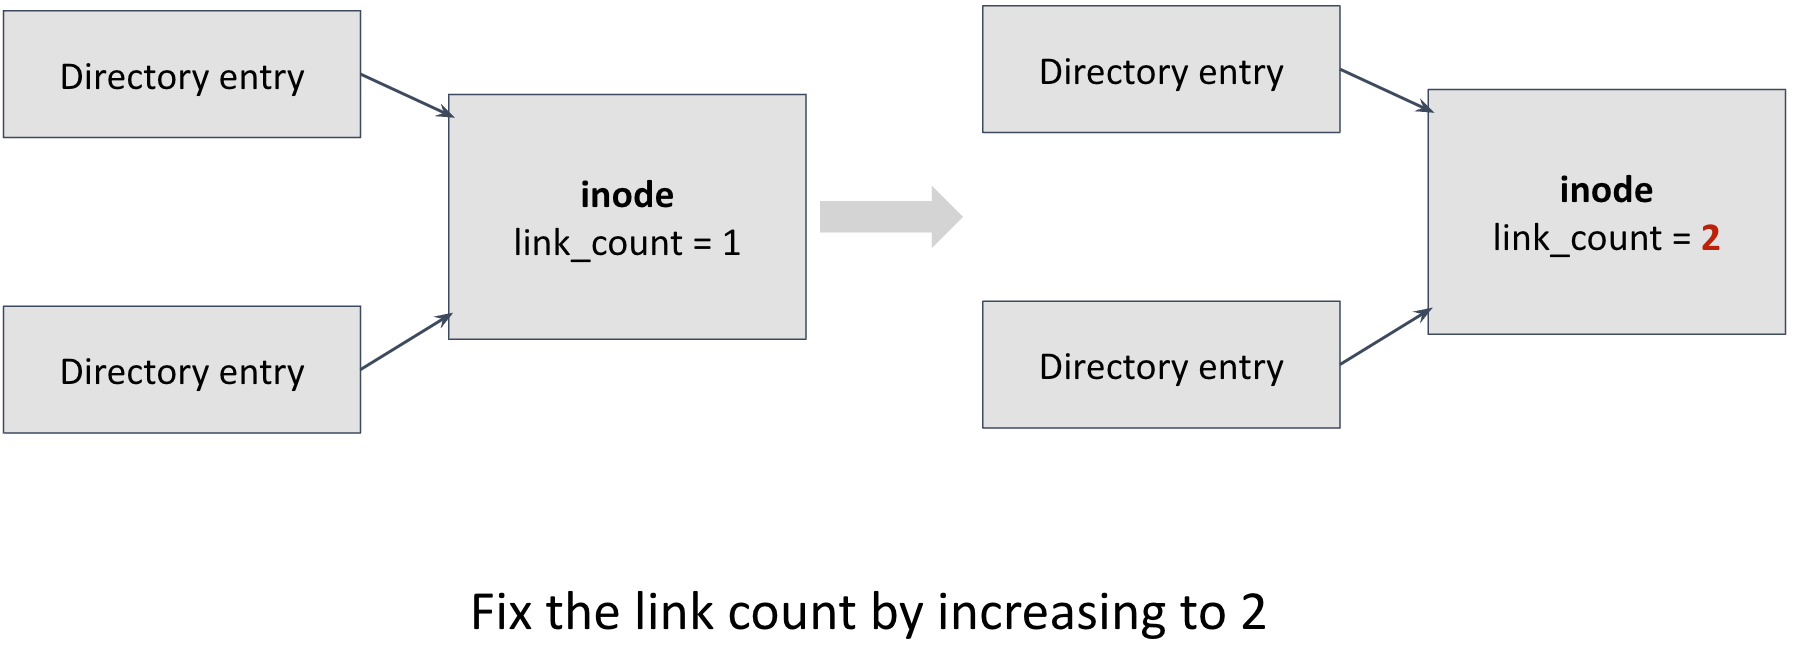
\includegraphics[width=0.8\textwidth]{chapters/L7/images/fsck-link.png}
    \end{center}
\newpage
    \item [-] \textbf{Lost Inodes:}
    If an inode has a link count greater than zero but no directory entries point to it, the \texttt{fsck} moves the corresponding file to the \texttt{lost+found} directory, allowing for potential recovery by the system administrator.
    \begin{center}
        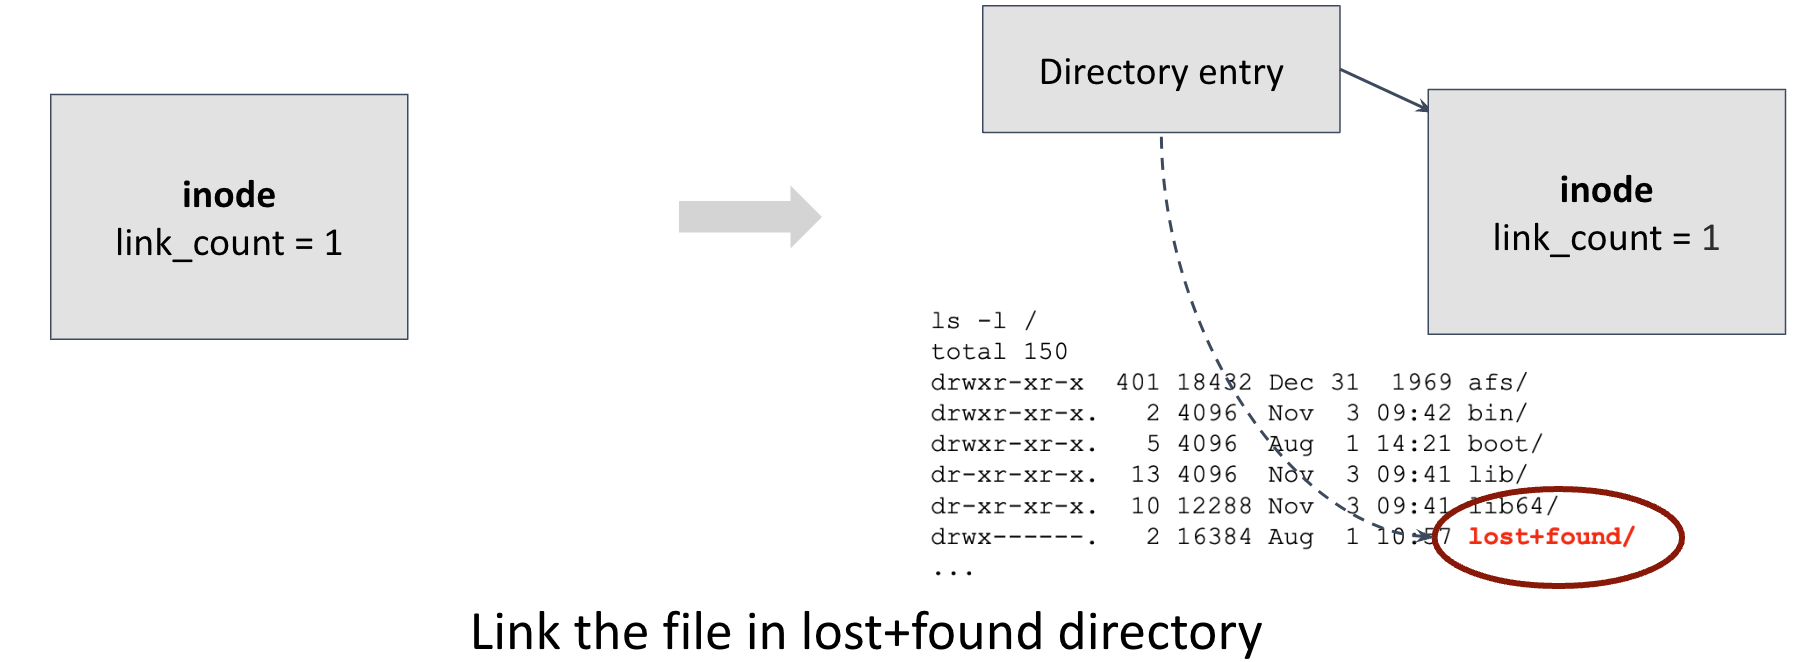
\includegraphics[width=0.8\textwidth]{chapters/L7/images/fsck-link2.png}
    \end{center}

    \item [-] \textbf{Data Bitmap Errors:}
    The \texttt{fsck} ensures the data bitmap accurately reflects the allocation status of blocks. If an inode points to a block, but the corresponding bit in the data bitmap is 0 (indicating the block is free), \texttt{fsck} corrects the bitmap to reflect the block's usage.
    \begin{center}
        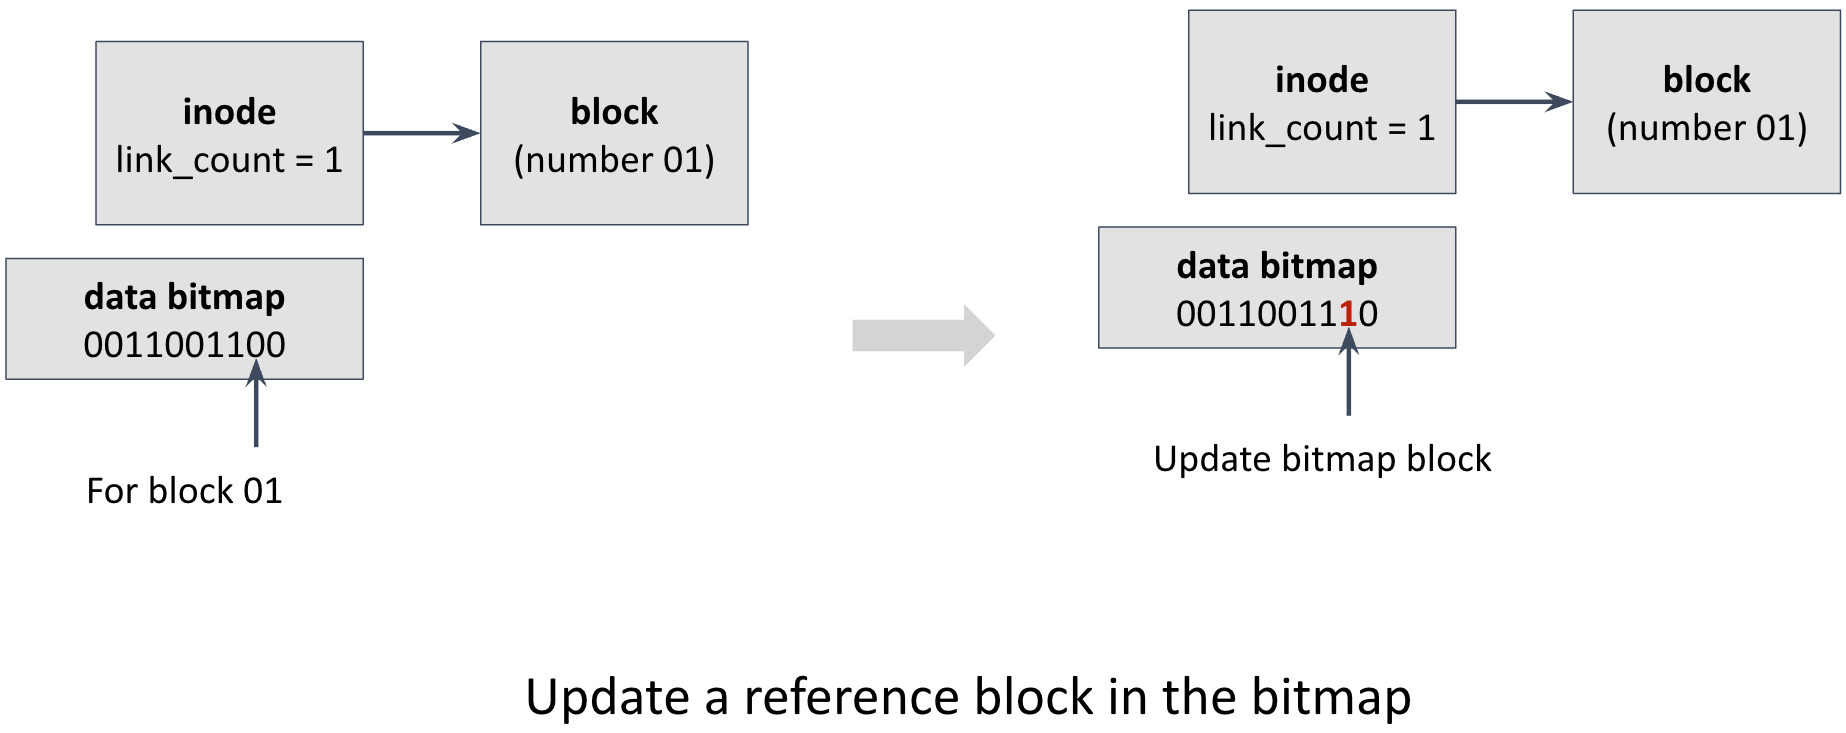
\includegraphics[width=0.8\textwidth]{chapters/L7/images/fsck-bitmap.png}
    \end{center}

    \item [-] \textbf{Duplicate Pointers:}
    The \texttt{fsck} identifies and resolves situations where multiple inodes point to the same data block, which can lead to data corruption. In such cases, \texttt{fsck} may create a duplicate of the block, updating one of the inodes to point to the new duplicate, thus preserving data integrity.
    \begin{center}
        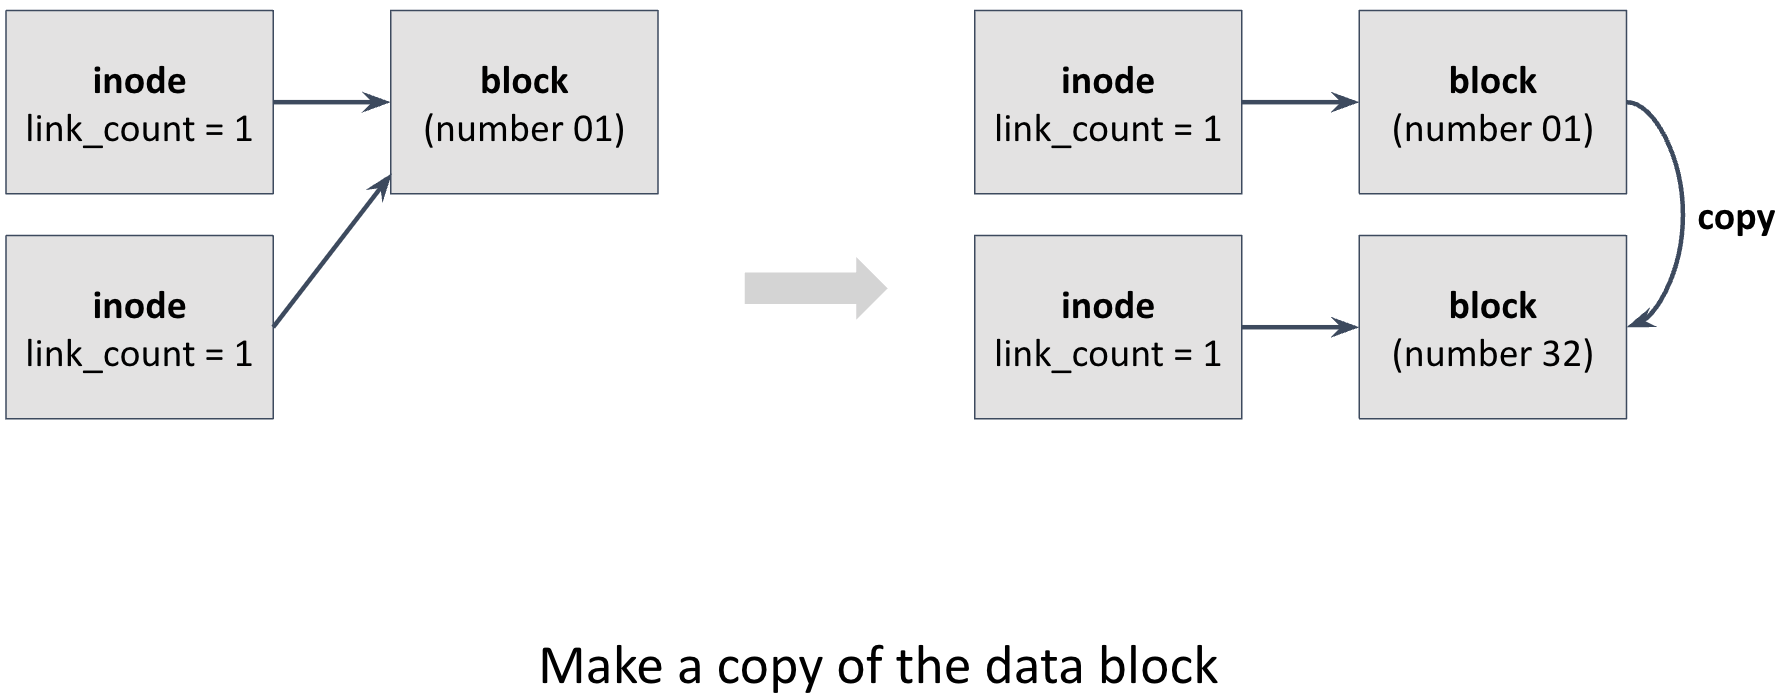
\includegraphics[width=0.8\textwidth]{chapters/L7/images/fsck-dupp.png}
    \end{center}
\newpage
    \item [-] \textbf{Invalid Pointers:}
    The \texttt{fsck} checks for inodes pointing to blocks with numbers exceeding the total number of blocks in the file system. Such pointers are invalid and can cause crashes or data corruption. The \texttt{fsck} removes these invalid pointers to prevent further issues.
    \begin{center}
        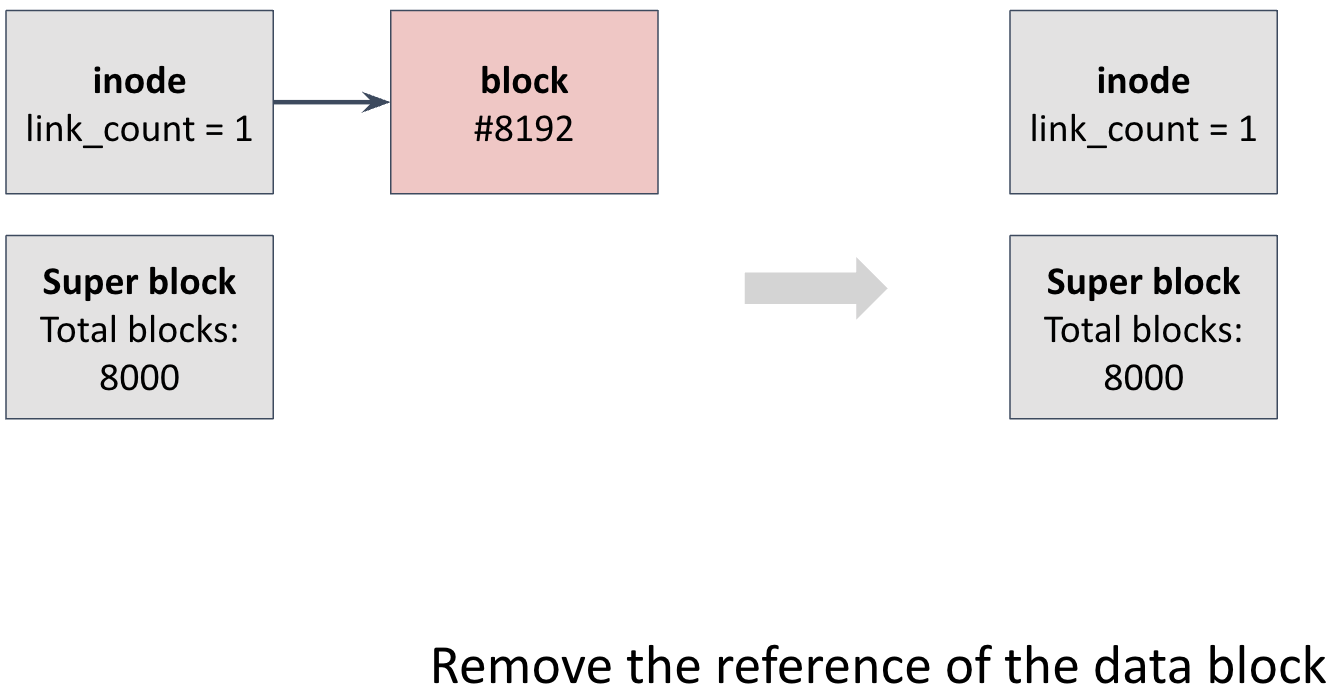
\includegraphics[width=0.8\textwidth]{chapters/L7/images/fsck-bad.png}
    \end{center}
\end{itemize}

\subsection{Problems with FSCK}

While \texttt{fsck} is essential, it has limitations:

\begin{itemize}
    \item [-] \textbf{Functionality:}
    \texttt{fsck} aims to bring the file system to a consistent state, which is not always the "correct" state. Determining the appropriate corrections can be challenging, and in severe cases, reformatting the disk may seem like the easiest solution, albeit with significant data loss.

    \item [-] \textbf{Performance:}
    \texttt{fsck} can be slow, sometimes taking hours to complete, especially on large file systems. This prolonged downtime can be disruptive.
\end{itemize}

\section{Consistency Solution \#2: Journaling}

To address the limitations of \texttt{fsck}, journaling offers an alternative approach to maintaining file system consistency with the following goals:

\begin{itemize}
    \item [-] Minimize the amount of work required for recovery after a crash.
    \item [-] Achieve the \textit{correct} state of the file system, not just a consistent one.
\end{itemize}

The core idea behind journaling is to record changes in a journal (or log) before applying them to the actual file system. This journal serves as a historical record of operations, allowing the system to recover to a known good state in the event of a crash. No need to scan the entire disk
\vspace{5px}
\begin{definition}[Journaling]
    Journaling is a technique used in file systems where all intended modifications are first recorded in a sequential log (the "journal") before being committed to the main file system. This write-ahead logging ensures atomicity and durability of operations, facilitating recovery after a crash.
\end{definition}
\vspace{5px}
Before modifying any data (read, write, delete, etc.), the changes are first recorded in the journal. The journal is a special area on the disk that stores data in a write-ahead fashion. Journaling leverages the atomicity of transactions to provide crash consistency.

\subsection{A Principled Approach: Transactions}

Journaling relies on the concept of transactions to ensure data integrity.

\begin{definition}[Transaction]
    A transaction is a group of operations treated as a single logical unit of work. It must adhere to the ACID properties: Atomicity, Consistency, Isolation, and Durability.
\end{definition}

\begin{itemize}
    \item [-] \textbf{Atomic:} A transaction is indivisible; either all operations within it are executed, or none are.
    \item [-] \textbf{Consistent:} A transaction must maintain the integrity of the data. It moves the system from one valid state to another.
    \item [-] \textbf{Isolated:} Concurrent transactions should not interfere with each other. The effects of one transaction should not be visible to others until it is complete.
    \item [-] \textbf{Durable:} Once a transaction is committed, its effects are permanent and survive system failures.
\end{itemize}

Transactions can have two outcomes:

\begin{itemize}
    \item [-] \textbf{Commit:} The transaction is successfully completed, and its changes are made permanent.
    \item [-] \textbf{Abort:} The transaction is terminated, and any changes made during the transaction are rolled back, restoring the system to its previous state.
\end{itemize}

\subsection{How Journaling Works}

Journaling groups file system operations into atomic and consistent units using transactions. \texttt{TxBeg} and \texttt{TxEnd} markers denote the start and end of a transaction. The process involves writing to the journal first and then writing the actual file system blocks (checkpoint) in a specific order. Journaling can be applied to both data and metadata blocks.

\begin{center}
    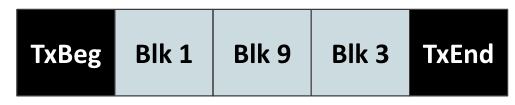
\includegraphics[width=0.45\textwidth]{chapters/L7/images/journal-record.png}
\end{center}

\subsection{Data Journaling: An Example}

Consider adding a new block \texttt{D2} to a file. This can be viewed as similar to operations in \texttt{git}. The steps involved in data journaling are:

\begin{enumerate}
    \item Write the following blocks to the journal: \texttt{TxBeg | Iv2 | Bv2 | D2 | TxEnd}. Here, \texttt{Iv2} represents the inode update, \texttt{Bv2} represents the bitmap information, and \texttt{D2} is the new data block. Writing each record to a separate block ensures atomicity.
    \item Write the blocks \texttt{Iv2}, \texttt{Bv2}, and \texttt{D2} to their respective locations in the file system (checkpoint).
    \item Mark the transaction as free in the journal (i.e., remove it).
\end{enumerate}

In case of a crash:

\begin{itemize}
    \item [-] If the crash occurs before the log is updated, the changes are ignored as if the transaction never happened.
    \item [-] If the crash occurs after the log is updated but before the checkpoint, the changes are replayed from the log back to the disk during recovery.
\end{itemize}

\subsection{Simplified Journaling Example}

Consider the goal of atomically writing the value 10 to block 0 and the value 5 to block 1.

\begin{center}
    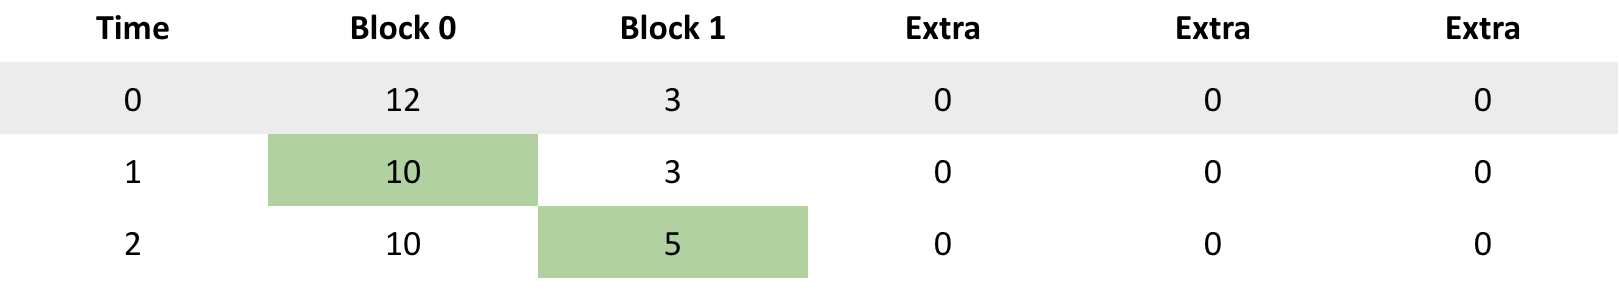
\includegraphics[width=0.9\textwidth]{chapters/L7/images/journal-example.png}
\end{center}

A naive approach of directly writing to the blocks is problematic because a crash between the two writes could leave the file system in an inconsistent state.

Journaling solves this by first writing the changes to the journal within a transaction.

\begin{center}
    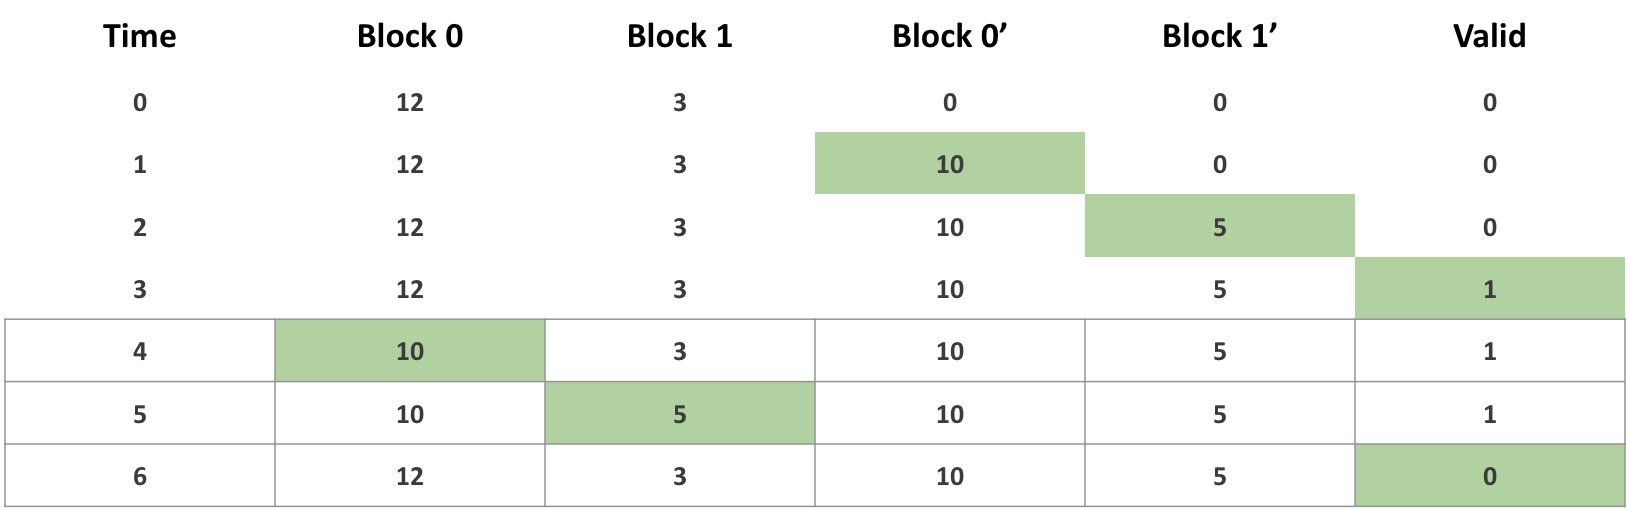
\includegraphics[width=0.9\textwidth]{chapters/L7/images/journal-example2.png}
\end{center}

The steps are as follows:

\begin{enumerate}
    \item Write the transaction begin marker (\texttt{TxBeg}) to the journal.
    \item Write the data for block 0 (value 10) to the journal.
    \item Write the data for block 1 (value 5) to the journal.
    \item Write a valid block indicator to the journal, signifying that the transaction completed successfully in the journal.
    \item Write the data for block 0 (value 10) to block 0 in the main file system.
    \item Write the data for block 1 (value 5) to block 1 in the main file system.
\end{enumerate}

\begin{center}
    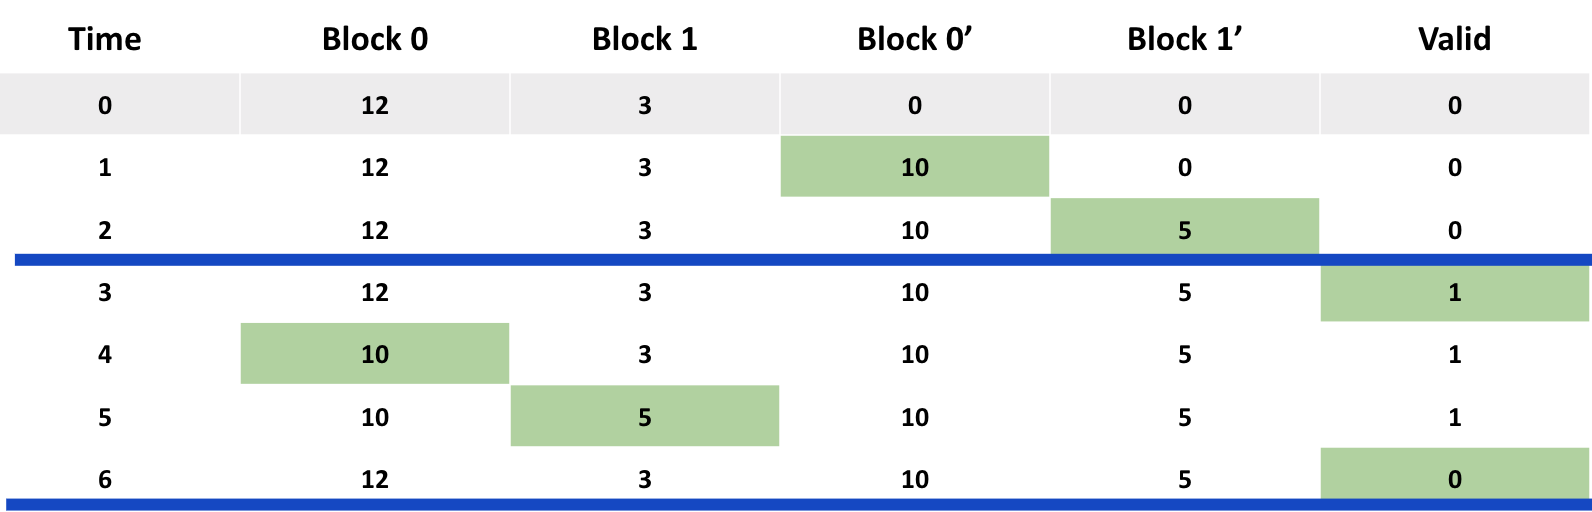
\includegraphics[width=0.9\textwidth]{chapters/L7/images/journal-example3.png}
\end{center}
\newpage
\textbf{Crash Scenarios:}

\begin{itemize}
    \item [-] \textbf{Crash before time unit 3:} The file system retains the old data, as the transaction was not fully written to the journal.
    \item [-] \textbf{Crash after time unit 3 but before time unit 6:} Upon recovery, the system detects the incomplete transaction in the journal and replays the changes to blocks 0 and 1, ensuring the new data is present.
    \item [-] \textbf{Crash after time unit 6:} The new data is already present in the file system, and no recovery is needed.
\end{itemize}
\end{document}